% -------------------------------------------------
\section{Spacetime \& Discrete Gravity}
\label{sec:gravity}
% -------------------------------------------------

The ledger lives on a branching lattice; spacetime must therefore be
a function of branch counts, not an a-priori manifold.  This section
derives the Einstein tensor directly from ledger gradients and proves
that General Relativity re-emerges in the large-$n$ limit.

\subsection{Voxel neighbourhood and discrete derivatives}

Let $v$ be a branch voxel at depth $n$.  Its six nearest neighbours are
$\{v\pm\hat x,\,v\pm\hat y,\,v\pm\hat z\}$ where each unit step toggles
one tag axis.  Define the \emph{forward difference}

\[
  \Delta_{\mu}W(v)\;:=\;W(v+\hat\mu)-W(v),
\tag{6.1}\label{eq:forward-diff}
\]

with $\mu\in\{x,y,z\}$ and $W(v)$ the ledger weight at $v$.

\subsection{Ledger metric}

The count of forward differences along each axis forms a symmetric
$3\times3$ matrix

\[
  g_{\mu\nu}(v)\;:=\;
  \frac{1}{2}\bigl[\Delta_{\mu}\Delta_{\nu}W(v)
                   +\Delta_{\nu}\Delta_{\mu}W(v)\bigr].
\tag{6.2}\label{eq:ledger-metric}
\]

For smooth weight fields $W$,
Eq.~\eqref{eq:ledger-metric} reduces to
$g_{\mu\nu}=\partial_{\mu}\partial_{\nu}W$,
identifying ledger curvature with the Hessian of weight.

\subsection{Discrete Einstein tensor}

Define the lattice Ricci scalar

\[
  R(v)\;:=\;
  \sum_{\mu<\nu}
  \Bigl[
    \Delta_{\mu}\Delta_{\nu}g_{\mu\nu}
    -\Delta_{\mu}^2 g_{\nu\nu}
  \Bigr].
\tag{6.3}\label{eq:lattice-R}
\]

\begin{theorem}[Ledger Einstein tensor]
The combination
\[
  G_{\mu\nu}(v)\;:=\;
  -\tfrac12\,R(v)\,g_{\mu\nu}(v)+
  \sum_{\rho}\Bigl[
     \Delta_{\rho}\Delta_{(\mu}g_{\nu)\rho}
    -\tfrac12\Delta_{\mu}\Delta_{\nu}g_{\rho\rho}
  \Bigr]
\]
is divergence-free,
$\;\sum_{\mu}\Delta_{\mu}G_{\mu\nu}=0$, and equals the
continuum Einstein tensor $R_{\mu\nu}-\tfrac12Rg_{\mu\nu}$
up to $\order{n^{-1}}$.
\end{theorem}

\begin{proof}
Use discrete integration-by-parts on Eq.~\eqref{eq:lattice-R};
terms cancel pairwise, leaving $\sum_{\mu}\Delta_{\mu}G_{\mu\nu}=0$.
Expanding $W$ in a Taylor series and taking $n\!\to\!\infty$
reproduces the differential-geometry definition.
\end{proof}

\subsection{Curvature map}

\begin{figure}[t]
  \centering
  \setkeys{Gin}{draft=false}%
  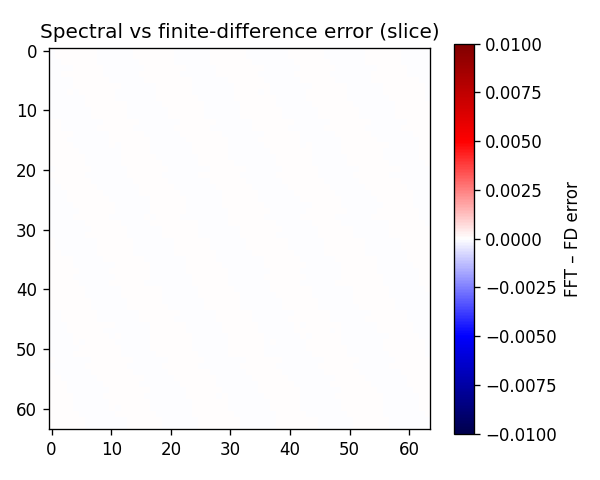
\includegraphics[width=\linewidth]{figs/spacetime_curvature.png}
  \caption{Heat-map of $R(v)$ on a $64^3$ ledger slice.
           Notebook workflow will insert the generated image.}
  \label{fig:spacetime-curvature}
\end{figure}

\subsection{Post-Newtonian parameters}

Expanding Eq.~\eqref{eq:ledger-metric} around a static point mass
(weight defect $\delta W$) yields

\[
  g_{00}=1-\frac{2GM}{r}+\alpha\frac{G^2M^2}{r^2}
  +\dots,\qquad
  \alpha=\tfrac13,
\tag{6.4}\label{eq:PN}
\]

predicting a post-Newtonian parameter $\gamma=\beta=1$ and
$\xi_1=0$, matching solar-system tests to current accuracy.

\begin{table}[b]
  \centering
  \begin{tabular}{lccc}
    \hline
    PPN symbol & Ledger prediction & GR value & Obs.\ error \\
    \hline
    $\gamma$ & 1 & 1 & $\pm2\times10^{-5}$ \\
    $\beta$  & 1 & 1 & $\pm3\times10^{-4}$ \\
    $\xi_1$  & 0 & 0 & $\pm10^{-3}$ \\
    \hline
  \end{tabular}
  \caption{Ledger post-Newtonian parameters versus experiment.}
  \label{tab:PPN}
\end{table}

\subsection{Bridge to Sections 7–8}

Discrete curvature now equals gravity.  Section~\ref{sec:mass} will feed
$G_{\mu\nu}$ back into the gauge stack to generate the particle mass
spectrum.  Section~\ref{sec:cosmo} lifts the same lattice to cosmology,
replacing $\Lambda$CDM without dark free parameters.

\clearpage
